\documentclass[a4paper,11pt]{article}
\usepackage{geometry}
 \geometry{
  a4paper,
  total={160mm,247mm},
  left=25mm,
  top=25mm,
 }
\usepackage[T1]{fontenc}
\usepackage[polish]{babel}
\usepackage[utf8]{inputenc}
\usepackage{fancyhdr, lipsum, setspace, amsmath, array, multirow, color, colortbl, listings, graphicx, MnSymbol, xcolor, float, multicol, ragged2e, algorithm2e, hyperref}

\pagestyle{fancy}
\fancyhf{}
\lhead{R. Makowski, K. Osada, M. Regulski, K. Tatarynowicz}
\rhead{Dokument projektowy}
\cfoot{\thepage}
\setlength{\headheight}{14pt}

\hypersetup{
  colorlinks  = true,
  linkcolor   = black,
  citecolor   = black,
  urlcolor    = blue
}
\urlstyle{same}

\onehalfspacing
\frenchspacing
\author{Remigiusz Makowski, Krzysztof Osada, Marcin Regulski, Krzysztof Tatarynowicz}
\title{\textbf{\Huge{Metody wytwarzania oprogramowania}}\\[3pt] Dokument projektowy}
\begin{document}
  \singlespacing
    \maketitle\thispagestyle{empty}
  \onehalfspacing
  \section{Temat realizowanego projektu}
    Aplikacja „TO-DO” oferująca (w podstawowej wersji) dodawanie, usuwanie i modyfikowanie notatek .
  
  \section{Skład grupy projektowej}
  \begin{enumerate}
    \item Remigiusz Makowski 
    \item Krzysztof Osada 
    \item Marcin Regulski 
    \item Krzysztof Tatarynowicz 
  \end{enumerate}
    
  \section{Specyfikacja wymagań}
  \begin{enumerate}
    \item System umożliwia użytkownikom zarządzanie notatkami ,,To-Do''.
    \item Użytkownik ma możliwość dodawania notatek do własnej listy, edycji oraz usuwania notatek. 
    \item Użytkownik uzyskuje dostęp do systemu poprzez dowolną przeglądarkę internetową. 
    \item System zapewnia użytkownikowi łatwy, wygodny i nowoczesny interfejs graficzny -- niezależnie od wybranej przeglądarki. Układ ten jest w pełni responsywny. 
    \item System zapewnia przejrzysty i poprawnie działający interfejs na urządzeniach mobilnych. 
    \item System gwarantuje bezpieczeństwo notatek użytkownika. 
    \item System posiada mechanizm rozpoznawania użytkowników. Mechanizm ten opiera się na unikalnych identyfikatorach oraz haśle dostępu. 
    \item System umożliwia synchronizację danych z wybranymi serwisami społecznościowymi (np. Google Calendar, Facebook).
    \item System działa w oparciu o nowe technologie. 
    \item System posiada możliwość łatwej rozbudowy o dodatkowe komponenty.
  \end{enumerate}

  \section{WBS} 
  Znajduje się pod adresem:\newline
  \url{https://raw.githubusercontent.com/krymeer/mwo/master/zadania/WBS/WBS.png}.

  \section{Wstępny harmonogram projektu}
  \begin{enumerate}
    \item Ramowy podział zadań -- do 24 października. 
    \item Zapewnienie działania podstawowych funkcjonalności (front-end, back-end, dodawanie, usuwanie, modyfikowanie notatek itd.) -- do 13 listopada. 
    \item Dołączenie ewentualnych rozszerzeń -- do 27 listopada. 
    \item Przetestowanie działania aplikacji -- do 30 listopada. 
    \item Zakończenie projektu zespołowego -- do 8 grudnia.
  \end{enumerate}

  \section{Cechy charakterystyczne wybranych technologii}
  \begin{enumerate}
    \item CSS, HTML -- języki wykorzystywane do budowania statycznych stron internetowych. Pierwszy z nich służy do tworzenia list dyrektyw i reguł określających, jak ma być wyświetlana dana witryna, drugi zaś odpowiada za podział strony na mniejsze części („szkielet”). 
    \item CSS Grid Layout -- moduł CSS3 umożliwiający swobodne dzielenie bloków strony internetowej na mniejsze, prostokątne fragmenty. Jego innowacyjność bierze się stąd, że dotychczas taki podział był możliwy jedynie w jednym wymiarze. 
    \item Vue.js -- kompaktowy framework upraszczający budowanie interfejsów aplikacji webowych, ze szczególnym naciskiem na reaktywność interfejsu. W przeciwieństwie do głównych konkurentów -- Angulara i Reacta -- Vue nie narzuca całej struktury aplikacji. Ma też znacznie mniejsze API, dzięki czemu jest łatwiejszy do przyswojenia. 
    \item ServiceWorker -- skrypt uruchamiany przez przeglądarkę w tle (w odróżnieniu od strony internetowej). Działa jako proxy pomiędzy stroną a przeglądarką i siecią, pozwalając m.in. na tworzenie aplikacji działających w trybie offline. 
    \item DynamoDB -- nierelacyjna baza danych zapewniająca dostęp do informacji w bardzo krótkim, milisekundowym czasie  w każdym rozmiarze. Co więcej, ma wiele zautomatyzowanych funkcji i jest elastyczna.
  \end{enumerate}

  \section{Uzasadnienie, dlaczego dana technologia powinna znaleźć się w\,projekcie}
  \begin{enumerate}
    \item CSS, HTML -- podstawa nowoczesnych stron WWW.
    \item CSS Grid Layout -- jest nowoczesnym modułem i znacząco ułatwia dzielenie stron na mniejsze fragmenty.
    \item Vue.js pozwala w prosty i uporządkowany sposób zarządzać przepływem informacji w interfejsie użytkownika. W porównaniu do innych frameworków jest lżejszy i prostszy w obsłudze; wartość dodana (w stosunku do nieużywania frameworka) to zapewnienie jednolitego mechanizmu obsługi reakcji interfejsu na zmiany w danych (data binding).
    \item ServiceWorker umożliwi korzystanie z aplikacji nawet wtedy, kiedy sieć internetowa nie jest w ogóle dostępna. Taka funkcjonalność może stanowić jedną z cech wyróżniających projekt. 
    \item DynamoDB - szybkość działania oraz kontrola poprzez komendy w języku JavaScript, z\,którego projekt w dużej mierze korzysta. Mniejszy początkowy narzut pracy w stosunku do tradycyjnych baz relacyjnych. 
  \end{enumerate}

  \section{Projekt systemu z przykładowymi diagramami UML}

  \begin{figure}[h!]
    \begin{center}
      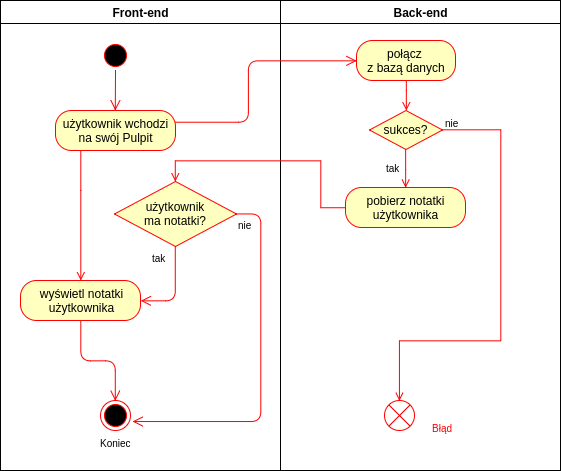
\includegraphics[width=0.5\textwidth]{../diagramy/diagram_stanow_1.png}
    \end{center}
    \caption{diagram aktywności: wyświetlenie notatek użytkownika}
  \end{figure}

  Projekt jest zrealizowany poprzez aplikację webową, którą generalnie można podzielić na dwie warstwy: front-end, obsługujący zdarzenia wywoływane od użytkownika, gromadzi dane i wyświetla interfejs graficzny, a także back-end, służący do komunikacji z serwerem, utrwalania notatek, autoryzacji użytkownika, przechowywania danych na jego temat itd.\newline

  \noindent Dodatkowy diagram projektu znajduje się pod adresem:\newline\url{https://github.com/krymeer/mwo/blob/master/zadania/diagramy/architektura.pdf}

  \begin{figure}[h!]
    \begin{center}
      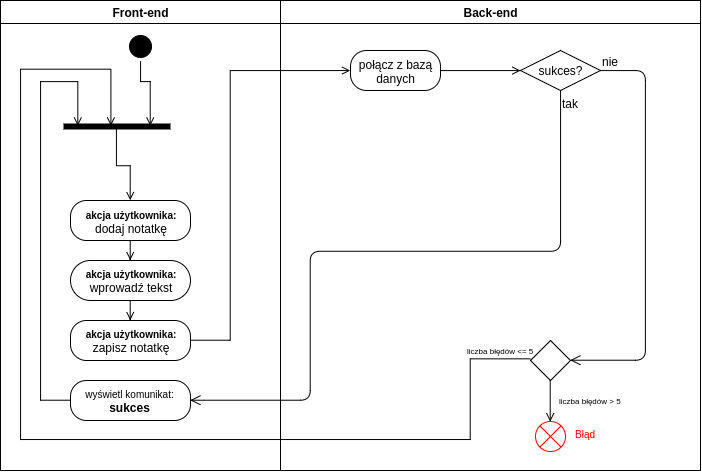
\includegraphics[width=0.5\textwidth]{../diagramy/diagram_stanow_2.png}
    \end{center}
    \caption{diagram aktywności: dodanie notatki użytkownika}
  \end{figure}


  \section{Wyszczególnienie ryzyk projektowych wraz z ich planami naprawczymi i metodami zapobiegania}
  
    \subsection{Brak czasu}
      \noindent\textbf{Opis:} Niewystarczająca ilość czasu na zrealizowanie wszystkich celów i wdrożenie zaplanowanych funkcjonalności.
      
      \noindent\textbf{Rozwiązanie:} zmniejszenie listy prac do wykonania, zredukowanie funkcjonalności aplikacji do tych koniecznych czy najistotniejszych.
      
      \noindent\textbf{Zapobieganie:} rozwijanie systemu na bieżąco, regularna kontrola postępu prac.

    \subsection{Awaria systemu}
      \noindent\textbf{Opis:} wystąpienie błędów w działaniu aplikacji spowodowanych wprowadzonymi w niej zmianami.
      
      \noindent\textbf{Rozwiązanie:} przywrócenie ostatniej sprawnej wersji systemu (przechowywanego na repozytorium).
      
      \noindent\textbf{Zapobieganie:} sprawdzanie działania systemu po każdej zmianie oraz eliminowanie w porę ewentualnych usterek.

    \subsection{Niewystarczające zasoby ludzkie}
      \noindent\textbf{Opis:} jeden (lub więcej) członków zespołu projektowego nie może lub odmawia wykonywania dalszych prac nad aplikacją.
      
      \noindent\textbf{Rozwiązanie:} przypisanie nieprzydzielonych zadań innym uczestnikom, ograniczenie liczby prac do wykonania w projekcie, ewentualnie znalezienie nowych współpracowników.
      
      \noindent\textbf{Zapobieganie:} ciągłe dbanie o motywację do działania każdego członka zespołu, skłanianie uczestników do systematycznej pracy.

    \subsection{Trudności implementacyjne}
      \noindent\textbf{Opis:} zaplanowane zadanie jest niemożliwe do zrealizowania bądź znacząco przekracza umiejętności wdrażającej je osoby.

      \noindent\textbf{Rozwiązanie:} w drugim przypadku -- przypisanie zadania innemu członkowi zespołu, w pierwszym -- znalezienie alternatywnego rozwiązania lub bezterminowe zawieszenie wykonywania zadania.
      
      \noindent\textbf{Zapobieganie:} rzetelnie sprawdzanie zarówno możliwości używanych technologii, jak i korzystających z nich członków zespołu.

  \section{Podział prac implementacyjnych na dwie trzytygodniowe iteracje}
    \subsection{Iteracja pierwsza}
      \textbf{Czas trwania:} 23 października -- 12 listopada 2017 roku
      \begin{itemize}
        \item zaprojektowanie systemu;
        \item przydzielenie zadań uczestnikom projektu;
        \item zaimplementowanie podstawowej funkcjonalności, tj. dodawania, usuwania i modyfikowania notatek, zakładania kont użytkowników, zapewnienia bezpieczeństwa danych;
        \item testowanie bazowej funkcjonalności pod kątem poprawności i efektywności działania, szukanie ewentualnych błędów;
        \item wybór najważniejszych zadań do wykonania w drugiej iteracji.
      \end{itemize}
    \subsection{Iteracja druga}
      \textbf{Czas trwania:} 13 listopada -- 3 grudnia 2017 roku
      \begin{itemize}
        \item ponowne omówienie projektu i podzielenie prac na uczestników;
        \item zaimplementowanie dodatkowych funkcjonalności, takich jak: rozszerzenie do przeglądarki, pobieranie danych z zewnętrznych systemów (JSOS, Facebook, Google itp.) czy udostępnianie wydarzeń;
        \item próba wdrożenia nowoczesnych technologii chmurowych;
        \item wprowadzenie przykładowych danych do systemu;
        \item testowanie aplikacji po wprowadzeniu każdej większej zmiany;
        \item zaproszenie osób trzecich do sprawdzenia działania systemu;
        \item opracowanie ewentualnej dokumentacji lub samouczka objaśniającego, jak należy korzystać z aplikacji;
        \item zarchiwizowanie zbędnych plików, folderów i innych danych;
        \item podsumowanie wykonanych działań i wyciągnięcie ewentualnych wniosków.
      \end{itemize}
\end{document}